\RequirePackage[T1]{fontenc}
\documentclass[11pt,a4paper,journal,onecolumn]{IEEEtran}
\usepackage[a4paper,margin=25mm,headheight=14bp,headsep=6mm,footskip=11mm]{geometry}
\usepackage{fontspec}
\setmainfont{Times New Roman}[SmallCapsFeatures={Letters=SmallCaps}]
\usepackage{graphicx,amsmath,amssymb,array,booktabs,tabularx,xurl}
\usepackage[unicode,hidelinks,pdfencoding=auto]{hyperref}
\hypersetup{pdftitle={IS6400 Report Layout Sample v2},pdfauthor={Team Six Sigma},pdfsubject={Single-column IEEEtran course layout sample}}
\urlstyle{same}
\makeatletter
\renewcommand\normalsize{\fontsize{11bp}{22bp}\selectfont}
\renewcommand\small{\fontsize{11bp}{22bp}\selectfont}
\renewcommand\footnotesize{\fontsize{11bp}{22bp}\selectfont}
\def\ps@sample{\def\@oddhead{\normalfont\fontsize{11bp}{13bp}\selectfont IS6400\hfil Layout Sample v2}\let\@evenhead\@oddhead\def\@oddfoot{\normalfont\fontsize{11bp}{13bp}\selectfont\hfil\thepage\hfil}\let\@evenfoot\@oddfoot}
\newcommand{\tablecap}[1]{\begingroup\def\@captype{table}\caption{#1}\endgroup}
\newcommand{\figurecap}[1]{\begingroup\def\@captype{figure}\caption{#1}\endgroup}
% Course convention: full Figure/Table in prose; only caption labels are bold.
\long\def\@makecaption#1#2{%
 \vskip\abovecaptionskip
 \begingroup\normalsize
 \def\sampletable{table}%
 \ifx\@captype\sampletable
  \centering\textbf{Table \Roman{table}.}\par
  \textsc{#2}\par
 \else
  \noindent\textbf{Fig. \arabic{figure}.}\ #2\par
 \fi
 \endgroup\vskip\belowcaptionskip
}

\renewenvironment{thebibliography}[1]{\normalsize\list{[\arabic{enumiv}]}{\setlength{\labelwidth}{15bp}\setlength{\labelsep}{5bp}\setlength{\leftmargin}{20bp}\setlength{\itemsep}{5bp}\setlength{\parsep}{0pt}\usecounter{enumiv}}\raggedright\sloppy}{\endlist}
\makeatother
\setlength{\parindent}{1em}
\setlength{\parskip}{0pt}
\setlength{\tabcolsep}{5bp}
\renewcommand{\arraystretch}{1}
\setlength{\abovedisplayskip}{8bp}
\setlength{\belowdisplayskip}{8bp}
\setlength{\abovedisplayshortskip}{6bp}
\setlength{\belowdisplayshortskip}{6bp}
\widowpenalty=10000\clubpenalty=10000
\emergencystretch=1em
\begin{document}
\normalsize\pagestyle{sample}
\begin{center}
\vspace*{21mm}
{\fontsize{14bp}{22bp}\selectfont IS6400 Business Data Analytics\par}
\vspace{13mm}
{\fontsize{24bp}{30bp}\selectfont Finding Repeat Buyers\\with Limited Capacity\par}
\vspace{5mm}
{\fontsize{14bp}{22bp}\selectfont Prediction and Customer Segmentation on Olist\par}
\vspace{15mm}
{\fontsize{14bp}{22bp}\selectfont Team Six Sigma\par}
\vspace{5mm}
\begin{tabular}{cc}
CHEN Hanyu & LI Binxiong\\
LIU Xiuqi & LIU Yuwei\\
SUN Bo & YE Yuhan
\end{tabular}
\vspace{18mm}
\par Report Layout Sample v2\\
27 November 2026\\
A4 \textbullet\ Single column \textbullet\ 11 pt \textbullet\ Double spacing
\end{center}
\clearpage
\begin{center}\textsc{Executive Summary}\end{center}
This project studies how an online retailer can identify existing customers who are more likely to buy again when the team can contact only a limited number of people. We use the Olist transaction dataset to construct customer snapshots from information available before each prediction date. A future 90-day window records whether each customer makes another qualifying purchase.

The main analysis ranks eligible customers and compares lists of the same size. Customer segmentation adds a second view: it describes the kinds of customers included in the list and the groups that receive fewer places. This can help the business understand coverage and develop content ideas for later testing.

This sample illustrates one additional development comparison completed on 26 November. Three fixed weighted logistic-regression configurations use the same October training snapshot and January development snapshot. Each selects 2,937 customers from 29,368 candidates. The base configuration finds 50 repeat buyers; the delivery and review configurations find 49 and 48. These added fields do not improve the primary hit count in this comparison. The full report will present the wider model comparisons and later-period evidence alongside this result.

Probability calibration and value ranking remain separate extensions because they answer different questions and use their own experimental protocol. The practical recommendation is to use the ranking and group profiles as decision support, then evaluate any proposed contact content through a controlled business experiment. Historical purchase outcomes alone do not establish that contacting a customer causes an extra purchase.

\vspace{5mm}\noindent\textit{Layout sample: the following pages contain selected, source-backed project material to demonstrate the agreed report format.}
\clearpage
\section{Introduction}
Olist provides a useful setting for studying repeat purchasing because its transaction records connect customers with orders over time~\cite{olist}. A retailer working with these records must decide where to spend limited attention. Contacting every previous buyer may be impractical, while a short list still needs to contain enough customers who are likely to return.

Our project combines prediction with customer segmentation. Prediction produces an ordered list. Segmentation describes groups of customers with similar characteristics and helps explain the list's coverage. The two outputs support different parts of the business decision: whom to prioritise, and how to understand the people selected or missed.

\section{Problem Statement}
The main question is: among eligible existing customers at a prediction date, which customers should receive the available places? The analysis compares methods at the same capacity so that a larger list does not automatically appear better. A 10\% list is a comparison setting in the experiment, rather than an established operating optimum.

Let $S_K$ denote the $K$ customers selected by a method and let $y_i=1$ when customer $i$ makes a qualifying purchase in the next 90 days. The number of observed repeat buyers in that list is
\begin{equation}
H_K=\sum_{i\in S_K}y_i.
\label{eq:hits}
\end{equation}
Here, $H_K$ is a count of people, $K$ is the available list size, and $y_i$ is the observed outcome. Equation~\eqref{eq:hits} makes the business comparison concrete: at the same number of places, a method is useful if it identifies more of the customers who subsequently return.

The segmentation question is complementary: which groups receive places in the selected list, and which groups are less represented? A difference in coverage can suggest a business question even when adding a group label does not improve prediction. Any proposed content response then needs its own test.
\clearpage
\section{Data Description and Preparation}
One row represents a customer at a particular snapshot date. Historical features use the preceding six calendar months. The label records a qualifying order in the following 90 days, with the window's end excluded. An eligible event is an approved order with positive product value. Order items are first aggregated to orders, then linked to customers and summarised into snapshots.

Figure~\ref{fig:time} shows the two snapshots used in the additional field comparison. October has 21,160 training customers, including 211 repeat buyers. January has 29,368 development customers, including 230 repeat buyers. The January outcomes have already been examined during development; they are not a new blind test.

\begin{center}
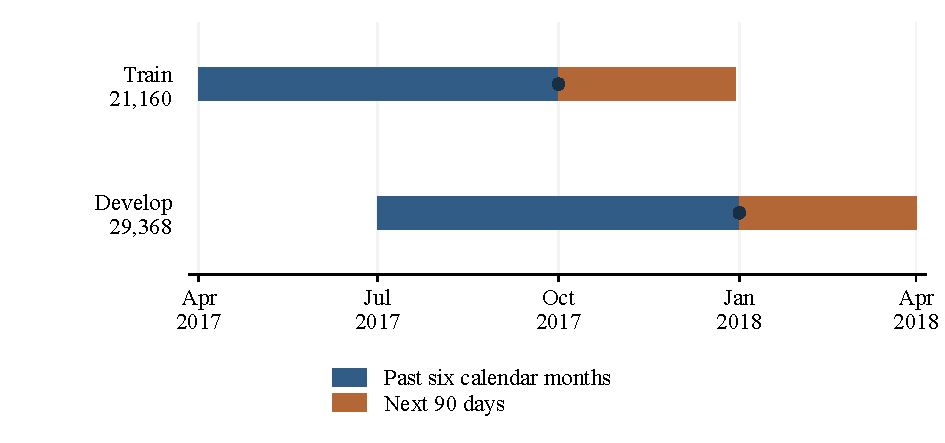
\includegraphics[width=\linewidth]{figures/time-windows.pdf}
\figurecap{Training and development windows for the fixed field comparison. A dot marks the snapshot date; blue denotes the historical feature window and orange the future label window. Counts refer to customer snapshots.\label{fig:time}}
\end{center}
The core fields describe recency, frequency, monetary value, average item rows, freight share, recent orders, recent spending and state. Imputation, scaling and category encoding are learned from the October training data. Delivery and review fields are restricted by their recorded availability at the snapshot date. Missing reviews are treated as missing information rather than as negative feedback.
\clearpage
\section{Methodology}
\subsection{Fixed Configurations}
F0 uses the eight core fields. G1 adds delivery fields; G2 adds review fields~\cite{experiment}. Table~\ref{tab:settings} gives their shared settings. The solver is limited-memory Broyden--Fletcher--Goldfarb--Shanno (L-BFGS).

\begin{center}
\tablecap{Shared Classifier Settings for F0, G1 and G2\label{tab:settings}}
\begin{tabularx}{\linewidth}{@{}lX@{}}\toprule
Setting & Value\\\midrule
Estimator & Logistic regression\\
Regularisation & Squared-coefficient (L2) penalty; inverse strength $C=1$\\
Solver & L-BFGS; tolerance $10^{-4}$\\
Class weighting & Balanced\\
Iteration limit / seed & 2,000 / 2026\\
Training / development & 1 October 2017 / 1 January 2018\\
\bottomrule\end{tabularx}
\end{center}
\subsection{Reading the Evaluation Measures}
Let $P$ be the number of repeat buyers in the full candidate pool. Two measures express different meanings of the hit count:
\begin{align}
\operatorname{Precision}@K&=\frac{H_K}{K},\label{eq:precision}\\
\operatorname{Recall}@K&=\frac{H_K}{P}.\label{eq:recall}
\end{align}
Using Equations~\eqref{eq:precision} and~\eqref{eq:recall}, F0 has $H_K=50$, $K=2{,}937$ and $P=230$. Precision is therefore 1.702\%: about 1.7 of every 100 selected customers repeat. Recall is 21.739\%: the list contains about 21.7\% of all repeat buyers in this candidate pool. These fractions describe observed purchase outcomes, not the causal effect of contacting customers.
\clearpage
\section{Experiment and Discussion}
Table~\ref{tab:results} compares the three fixed configurations at the same January capacity. Average precision (AP) summarises precision along the ranked list; the area under the receiver operating characteristic curve (ROC AUC) summarises discrimination across thresholds. Precision--recall analysis helps evaluate imbalanced data~\cite{saito2015}. These measures supplement the fixed-capacity hit count.

\begin{center}
\tablecap{January Development Results at $K=2{,}937$\label{tab:results}}
\begin{tabular}{@{}lrrrrr@{}}\toprule
Model & Hits & Precision (\%) & Recall (\%) & AP & ROC AUC\\\midrule
F0 & 50 & 1.702 & 21.739 & 0.0298 & 0.5817 \\
G1 & 49 & 1.668 & 21.304 & 0.0264 & 0.5857 \\
G2 & 48 & 1.634 & 20.870 & 0.0220 & 0.5898 \\
\bottomrule\end{tabular}
\end{center}
\begin{center}
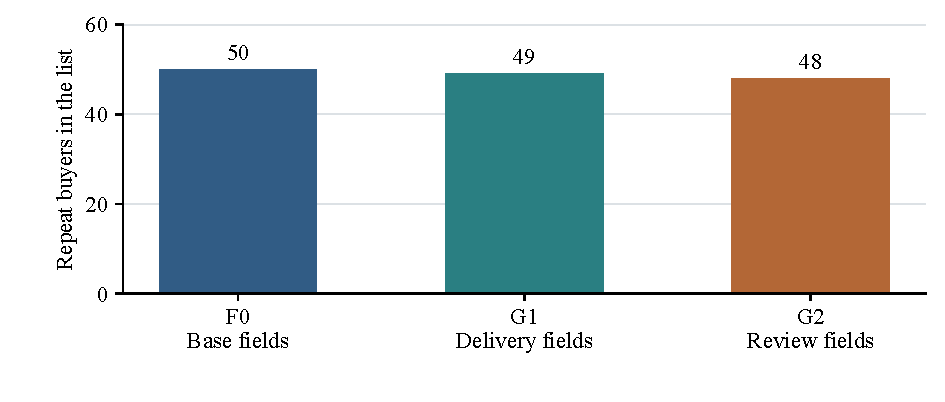
\includegraphics[width=\linewidth]{figures/feature-comparison.pdf}
\figurecap{Observed repeat buyers in three equal-sized development lists. All configurations use 29,368 January candidates and select 2,937 people; the vertical axis starts at zero. Source: the fixed F0/G1/G2 results~\cite{experiment}.\label{fig:comparison}}
\end{center}
Figure~\ref{fig:comparison} highlights the primary result: G1 and G2 find one and two fewer repeat buyers than F0. Their slightly higher ROC AUC does not translate into a higher hit count at this capacity. This is an additional development comparison; it does not establish statistical equivalence or performance in a new test period.
\clearpage
\section{Conclusion}
The selected experiment supports a limited, practical conclusion. Adding these delivery or review fields does not increase the number of repeat buyers found in the January top-10\% list. F0 remains the reference for this comparison. The full report will connect this result with the wider baseline comparisons, customer-group coverage and later-period checks.

The business can use the ranked list to allocate a fixed number of places and use group profiles to understand its composition. A later controlled content experiment can compare a general shopping guide with a topic-specific guide while keeping the contact policy clear. Claims about additional purchases or profit require an appropriate comparison and the relevant business costs.

Probability calibration and value ranking should be interpreted within their separate protocol. The report will keep their results distinct from the full-training ranking models, so that readers can see what changed in each comparison.

\vspace{3mm}\noindent\textit{Codex assisted with formatting and preparation of this layout sample.}

\section*{Appendix --- References}
\begin{thebibliography}{3}
\bibitem{olist} Olist, ``Brazilian E-Commerce Public Dataset by Olist,'' Kaggle. [Online]. Available: \url{https://www.kaggle.com/datasets/olistbr/brazilian-ecommerce} (accessed Nov. 27, 2026).
\bibitem{experiment} Team Six Sigma, ``Fixed F0/G1/G2 development comparison,'' experiment \texttt{repair-G1G2-20261126}, Nov. 26, 2026. [Online]. Available: \url{https://github.com/CercaTrovato/olist-repurchase-analysis/blob/main/report-prep/20261126/data/feature-experiment-results.csv} (accessed Nov. 27, 2026).
\bibitem{saito2015} T. Saito and M. Rehmsmeier, ``The precision-recall plot is more informative than the ROC plot when evaluating binary classifiers on imbalanced datasets,'' \textit{PLOS ONE}, vol. 10, no. 3, e0118432, 2015. doi: \url{https://doi.org/10.1371/journal.pone.0118432}.
\end{thebibliography}
\end{document}
